\section{Construct a purpose-preserving qualification instrument}
\subsection{Actual scientific ingredients and the new request}
The first public source is PEtab Select test case 0009, pinned to commit \nolinkurl{7b1a1528cee614e72f17eb82338472e7ba91d8de}. It describes the sixteen possible acetylation states of histone H4 and sixty-four conversion reactions. The supplied measurement table has 252 rows over fifteen observables, all at equilibrium. The original authors supplied the model, measurements, fitted nominal parameters and model-space declaration. The fixed common reverse rate \texttt{da\_b=1} is a legitimate normalization. This edition does not present it as a fitted error or invalidate the original study \cite{h4}.

The research team supplies four reuse requests and the acceptance contract. Three requests use H4; the fourth uses a different public source, Boehm\_JProteomeRes2014, pinned to \nolinkurl{c44d5ede9bf979db5aa8ae4e94fc31fba9776675}. That second package contains forty-eight finite-time measurement rows, sixteen distinct times and three relative observables. Its reference-simulation table is explicitly distinguished from observations. Inspecting that table is not a new nonlinear simulation or biological experiment \cite{boehm}.

The instrument is a bounded Python library with source inventory, a supported SBML/PEtab interpreter, generator construction, stationary prediction, clock-invariance witness, necessary dimension check and request qualification. Its dynamics scope is a closed, normalized, irreducible first-order conversion network with one constant unit-volume compartment and one condition. Broader inventory does not imply broader solver validity. Unsupported dynamics fail closed. There is no proprietary weight update, hidden scientific oracle or newly invented identifiability theorem.

\subsection{The transformation witness}
For the supported H4 model, let $x$ be the normalized state distribution, $x_0$ its supplied initial condition and $Q$ its source-derived generator:
\[
\dot x=Qx,\qquad \mathbf{1}^{\mathsf T}x=1,\qquad Qp=0.
\]
Let $c>0$ be normalized model-time units per requested physical-time unit, and let $t$ be a time in that physical unit. This hypothetical clock conversion gives
\[
(cQ)p=0,\qquad x_c(t)=\exp(cQt)x_0=x(ct).
\]
Thus the equilibrium remains the same under a clock conversion while a finite-time response generally changes. The witness identifies a missing physical-clock calibration for the \emph{new request}. It does not claim that all stationary quantities are unidentifiable or that $c$ is another estimated parameter of the original normalized fit.

The necessary dimension check is similarly limited. A normalized sixteen-state equilibrium has at most fifteen independent mean coordinates. Thirty-two motif factors plus the common basal acetylation rate form a thirty-three-parameter kinetic superset, so its equilibrium mean-map rank deficiency is at least eighteen. Replicates improve precision without adding independent mean coordinates. The selected eight-parameter fitted model is not rejected by this bound. A complete identifiability analysis, parameter uncertainty and biological validation remain separate obligations.

The calibrated mission uses the spectral relaxation scale
\[
\tau_{\mathrm{model}}=\left[\min_{\lambda\in\sigma(Q)\setminus\{0\}}(-\operatorname{Re}\lambda)\right]^{-1},\qquad
\tau_{\mathrm{physical}}\in[\tau_{\mathrm{model}}/c_{\max},\ \tau_{\mathrm{model}}/c_{\min}].
\]
This is the asymptotic exponential scale of the supplied model, not a measured half-life or a finite-time settling guarantee. The bounded implementation treats eigenvalues of magnitude at most $10^{-9}$ as numerical zero and requires requalification for materially different rate scales. The positive bounds on $c$ are explicitly assumed in this experiment; they do not constitute an observed calibration or a statistical confidence interval.

The full transformation witness retains six parts: the original useful reuse decision; the mistaken transfer of generic execution into scientific validity; the reason to remove that assumption; the source/request/evidence contract and executable witnesses; realization against the original public files; and falsifiers. It fails if it approves the unsupported physical prediction, rejects valid conditional equilibrium use, uses two realizations that do not preserve the original observations, or silently carries the H4 witness into a changed finite-time mission. It also fails as a commercial advantage if a competent alternative delivers the same outcome at equal or lower complete cost.

\begin{table}[H]\small
\begin{tabularx}{\linewidth}{@{}p{0.21\linewidth}p{0.34\linewidth}X@{}}\toprule
Mission & Required useful result & Boundary that must remain visible \\ \midrule
Equilibrium reuse & Complete stationary distribution and mean acetylation, conditional on the supplied fit. & Preserve valid use; necessary dimension bound does not settle full identifiability. \\
Physical clock & Two finite-time realizations with the same equilibrium; state the missing calibration. & Alternative clocks are hypothetical conversions, not new measurements or replacement fit parameters. \\
Added calibration & Propagate supplied positive conversion bounds to a model relaxation interval. & The calibration is explicitly assumed; the interval is not a confidence interval or measured half-life. \\
Changed source & Inventory the Boehm measurements, bind its evidence and withdraw the old witness. & Finite observation times and a declared unit do not establish general identifiability or physical truth. \\ \bottomrule
\end{tabularx}
\caption{Acceptance preserves both useful positive qualifications and justified limitations. A packet that rejects everything fails.}
\end{table}

Every record binds the exact request, five core source files and a separate complete evidence mapping covering all supplied files. The latter includes the model-space declaration and reference simulations. A pre-exposure correction added that complete evidence identity; the preceding source and freeze remain in history. Each record begins with empty authority and explicitly denies biological validation. A previous receipt cannot revive expired permission or supply a new mission's meaning.

\subsection{Development, freeze and fresh recipient transfer}
The instrument was constructed after the opportunity selection. E's small contract-to-invariants workflow already existed and is unchanged; it was not tuned on the later scientific scores. The developer used H4 during construction. A candidate dimension count initially omitted the common basal rate; it was corrected from thirty-two to thirty-three before freeze, with the earlier artifact and failed review retained. Eighteen development tests pass, including an independently assembled motif generator and numerical integration. Those are development checks, not fresh independent model families.

The final capsule is 48,797 bytes and contains four generic code/documentation/manifest members. It excludes scientific data, cached answers, protected cases and scorer internals. An existing source-verified lifecycle bridge transports the actual bytes; the new recipient receives the recovered capsule. All thirty-one local conformance checks pass. An ordinary library receives identical bytes and permissions. This demonstrates technical transport and local control behavior with synthetic identities. It establishes no graph-specific advantage, live ENS authentication or production admission.

\begin{table}[H]\small
\begin{tabularx}{\linewidth}{@{}p{0.19\linewidth}p{0.31\linewidth}X@{}}\toprule
Artifact / lineage & Origin and recipient state & What transfers, and what does not \\ \midrule
Public scientific packages & Original authors' models, observations, nominal fits and reference simulations. & Attributed input evidence; no new physical experiment or source-author endorsement. \\
E workflow v1 & Researcher-authored before the original development job; unchanged in both pilots. & Existing contract/invariant expertise, newly supplied to each E recipient; no model upgrade. \\
Contract probes v1 & Extracted during an unpaid development repair; received by the earlier software E+ arm. & Three executable assertions with bounded semantics; no paid-origin or universal retry claim. \\
Scientific instrument v1 & Constructed after S3 selection using H4; frozen before the new recipient campaign. & Generic scoped code and provenance, without source data, answers or protected cases. Optional R\&D, not paid-job learning. \\
Scientific recipient adapter & Fresh E+ receives actual recovered capsule bytes and writes a current packet adapter. & New access and source-specific integration; capsule unchanged, authority empty and mission acceptance fresh. \\
Nonlinear successor candidate & Identified as possible next work after the Boehm boundary. & No implemented general solver, validated new service, observed saving or production admission. \\ \bottomrule
\end{tabularx}
\caption{Capability lineage separates prior expertise, construction, transfer and the next unbuilt hypothesis. The scientific instrument and earlier contract helper are separate branches of the research history.}
\end{table}


The established workflow, final instrument, scientific protocol, private evaluator and exact participant messages are hash-bound before exposure. This improves on the supporting software pilot, whose participant messages were reconstructed from the transcript rather than precommitted verbatim. Separately initialized U, E and \Eplus\ receive the same sources, useful formulation, tools, acceptance and outer limits: 1,200 seconds, forty-eight successful logged operations and forty-five seconds per Python execution. U can implement ordinary algebra and construct its own helpers. \Eplus\ adds only the received instrument to E's established workflow.

The qualified formulation is supplied to all three configurations. This is deliberate: it tests execution and the recipient's increment once the structure is known. It does not test whether an enhanced enterprise is better at inventing that structure. The participants are actual hosted frontier-model agents, not deterministic substitutes. Exact API identity, reasoning setting, token usage and invoices remain unexposed. The matched envelope covers observable time and operations, not hidden compute. These agents are not a representative human-user sample.

A separately authored conventional implementation uses direct linear algebra, matrix exponentials and eigenvalues without importing the candidate. It is a competent construction with unmeasured construction expense, not a free commercial service. The acceptance oracle independently reconstructs reactions, uses a singular-value stationary nullspace and Poisson uniformization for transients. Thirteen negative controls are rejected. Source and changed-request checks are automated; scientific prose was also inspected after all recipients froze. This is separate internal evaluation, not external scientific replication.

\section{Fresh results: a useful instrument, no established increment}
\begin{table}[H]\centering\small
\begin{tabular}{@{}lrrrrr@{}}\toprule
Configuration & Accepted & Hosted seconds & Operations & Python calls & Complete cost \\ \midrule
U & 4/4 & 366.09 & 13 & 8 & Unknown \\
E & 4/4 & 390.90 & 16 & 10 & Unknown \\
E+ & 4/4 & 383.30 & 14 & 8 & Unknown \\
Conventional & 4/4 & Not matched & Not matched & Not matched & Unknown \\
\bottomrule\end{tabular}
\caption{Observed scientific campaign after all three recipients froze. Both request variants pass. Conventional construction was separate; its local function runtime is not compared with a hosted construction turn.}
\end{table}
The observed E--U and E+--E acceptance differences are both zero percentage points. No final mission fails. All logged Python executions exit successfully; inspection calls are included in the execution count. U, E and E+ add ten, thirteen and twelve tests respectively, beyond the common smoke test. Their complete final packets and reports remain frozen. These tests do not create additional independent mission families.

\begin{figure}[H]\centering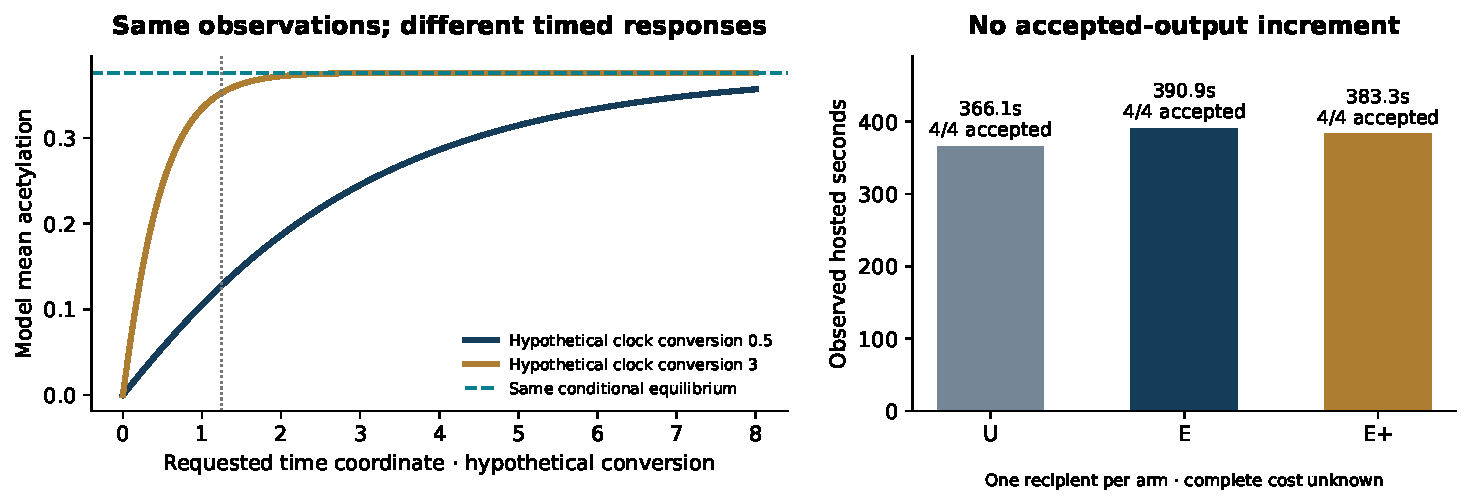
\includegraphics[width=0.97\linewidth]{figures/scientific_witness.pdf}\caption{Source-derived computational witness, not new biology. Clock conversions are hypothetical. At request time 1.25, the maximum state difference is 0.1433168 while the equilibrium agrees to numerical precision. The right panel reports single hosted observations, not a causal latency estimate.}\end{figure}
The accepted nominal model gives mean acetylation 0.3764225583 and a model spectral relaxation scale of 1.2815393182. Under the explicitly assumed conversion interval [0.4, 1.6] model units per minute, the propagated relaxation interval is [0.8009620739, 3.2038482954] minutes. It is a deterministic conditional interval, not measured biological timing or a confidence interval.



The accepted outcome is a source-bound computational qualification packet. The unknown physical conversion remains unknown; no amount of correct code creates a physical calibration. The calibrated request demonstrates useful conditional propagation after an additional assumption is supplied. It does not demonstrate experimental information gain. Boehm establishes a meaningful applicability boundary: the recipient uses shared inventory structure while withdrawing the old equilibrium witness. It does not show that the retained solver handles arbitrary nonlinear models.

H4 was seen during instrument development. Fresh recipient contexts and changed requests do not make its scientific source held out. Boehm is the fresh source family, and the four mission classes together form one campaign over two families. We do not calculate a confidence interval from eight deterministic request checks and describe it as evidence across eight independent opportunities. Public source availability also prevents a contamination-proof claim.

The capability-assisted recipient actually invokes the received inventory, stationary, dimension, clock and qualification functions without modifying their frozen bytes. This demonstrates usable transfer. All comparators already meet the same accepted requirements, so incremental accepted-output benefit is zero in this campaign. Observed hosted timing is descriptive and includes scheduling and generation. Complete accepted-output cost is unknown for every arm. A zero acceptance difference is neither general equivalence nor evidence that expert operation cannot matter elsewhere.

\section{Construct the arrangement as carefully as the capability}
\subsection{A service package with real missing inputs}
The candidate offering is a bounded scientific-model reuse qualification: one named source revision, one current requested quantity, a reproducible computation or witness, a source-bound decision and an explicit next evidence obligation. The natural counterparties are research software teams, core facilities and modeling consultancies. Their actual demand, willingness to pay and authority to share a generic adapter have not been observed.

Equivalent human service remains the primary commercial reference. No scope-matched quote was obtained for S3. For context only, Harvard Chan's published FY26 bioinformatics rates are \$193/hour for external academic institutions and \$265/hour for industry, including some computing and storage expense \cite{hbc}. That service primarily concerns sequencing analysis and is an analogy, not a quoted H4 qualification service or evidence that a prompt is worth those rates. The scoped human effort $h$ and applicable rate $r$ must be elicited for the same deliverable, deadline and customer effort before $H=hr$ is used to judge savings. We do not invent S3 revenue from this analogy.

The implemented arrangement checker represents the proposed capability, participant subset, outside options, mission values, uniform price, responsibilities, hypothetical rights, acceptance milestones, withdrawal, support, refunds, default and dates. It considers conventional delivery, instrument construction, coordinated commitments, their combination and HOLD. A conventional entrepreneur receives the entire same menu. There is no assumption that ordinary entrepreneurs cannot coordinate or use available tools.

The baseline technical benefit is \emph{zero} adaptation saving and zero quality uplift. A fifty-percent saving appears only as an explicitly unmeasured sensitivity. An independently useful common milestone is disabled unless the input explicitly asserts such usefulness. Required common construction is charged once in A, alongside its mission work; extra retention is B and optional additional exploration is C. Actual unpaid research is not relabeled as a purchased job. Arbitrary diagnostic dollars exercise the accounting mechanism; they are not estimates of S3's costs, values or prices.

\subsection{Expected contribution cannot finance an unfunded prefix}
For a dated scenario, let $C(t)$ denote cumulative net cash movement before opening capital, $E(t)$ refundable escrow liability, $S(t)$ support reserve and $R$ protected reserve. Required opening capital is
\[
L_{\min}=\max_t\{0,\ E(t)+S(t)+R-C(t)\}.
\]
The package must finance the maximum required across its declared scenarios. An escrow deposit increases cash and the refund liability equally, leaving available funds unchanged. Only actually earned and released payments can fund later work under these modeled terms. A delayed invoice or a default supplies no cash. Recognized revenue, collections, refunds, liabilities, reserves and profit are separate fields.

The executed finite grid has sixty configuration records and 4,320 candidate evaluations. Its zero-saving reference selects conventional delivery for P2 and P3 at the arbitrary diagnostic price of \$300 each with refundable escrow. Supplied scenario weights yield \$193.50 expected contribution, \$300 successful contribution, a \$40 worst named loss and \$230 required opening cash, including a \$50 reserve. These numbers are accounting-test conditions, not an S3 forecast. The new instrument is not selected in that reference. All sixty records permit an unrestricted conventional entrepreneur with the same menu; no technology-exclusive package is established.
\begin{table}[H]\centering\small
\begin{tabular}{@{}lrrr@{}}\toprule
Payment arrangement & Delay (days) & Opening cash & Success contribution \\ \midrule
After acceptance & 0 & \$470 & \$200 \\
After acceptance & 10 & \$840 & \$200 \\
Refundable escrow & 0 & \$470 & \$200 \\
Refundable escrow & 10 & \$840 & \$200 \\
Useful accepted milestone & 0 & \$370 & \$200 \\
Useful accepted milestone & 10 & \$840 & \$200 \\
\bottomrule\end{tabular}
\caption{Separate post-confirmation arithmetic illustration with fixed successful receipts and costs. A common milestone is assumed independently useful and accepted. Values are not buyer commitments or market estimates.}
\end{table}
\begin{figure}[H]\centering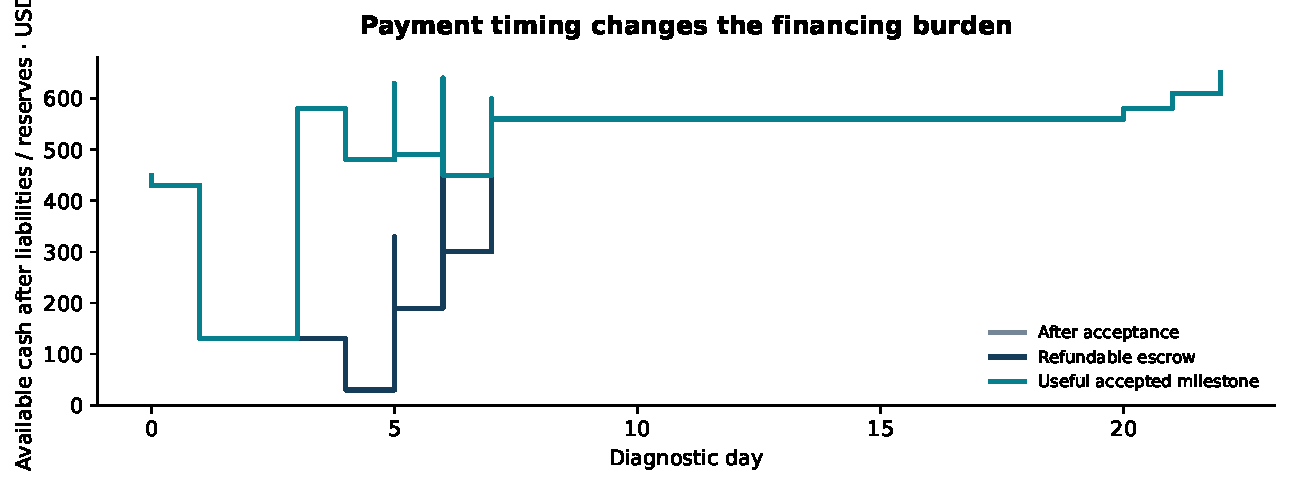
\includegraphics[width=0.97\linewidth]{figures/cash_timing.pdf}\caption{Arbitrary successful diagnostic paths with USD500 opening cash. Refundable principal remains unavailable. The separately useful accepted milestone requires less opening cash only when released early; all three arrangements need USD840 under the ten-day release delay. Identical successful contribution does not imply identical liquidity.}\end{figure}


Participation constraints compare each supplied expected net value with the participant's outside-option surplus. They are conditional inequalities, not proof that a coalition will form. The grid is finite, does not model every strategic bargaining deviation, and is not a market equilibrium. Common technical failure, withdrawal, partial acceptance, defaults and support are correlated through named scenarios rather than treated as independent successes. Seventeen of thirty-two fresh synthetic stress combinations lose money; all are retained. The observation that none exceeds the supplied opening-cash cap does not estimate real creditworthiness or loss probability.

The useful accepted common milestone in the timing illustration changes financing only if a buyer actually values it independently and releases payment in time. If it is merely a component of an unfinished promise, its payment cannot be assumed earned. The ordinary entrepreneur can offer the same legitimate milestone. Better arrangement design can matter without creating an exclusive technological advantage.

\section{What a successor can do next, and where to stop}
\begin{table}[H]\centering\small
\begin{tabular}{@{}p{0.29\linewidth}p{0.145\linewidth}p{0.145\linewidth}p{0.145\linewidth}p{0.15\linewidth}@{}}\toprule
Useful offering / boundary & U & E & E+ & Commercial margin \\ \midrule
Conditional H4 equilibrium & Pass & Pass & Pass & Unknown \\
Uncalibrated physical prediction & Evidence needed & Evidence needed & Evidence needed & Not qualified \\
Assumed-calibration propagation & Pass, conditional & Pass, conditional & Pass, conditional & Unknown \\
Fresh Boehm scope decision & Pass & Pass & Pass & Unknown \\
General nonlinear qualification & Not tested & Not tested & Not tested & Not established \\
\bottomrule\end{tabular}
\caption{Observed computational frontier under the frozen envelope. Pass means the scoped packet satisfies acceptance. No positive complete-cost commercial crossing is established. The refused physical prediction is different from the accepted explanation of why evidence is missing.}
\end{table}


The constructed asset lets another agent inventory a supported model, calculate the specified witness, package source-bound conditions, and recognize a changed mission that requires a different analysis. These are executable capabilities, not merely a summary in a graph. Their additional economic value remains unestablished because U, E and the conventional control deliver the same accepted result, full construction and serving costs are unknown, and buyers have not committed.

The next technical opportunity is mission-specific qualification of a genuinely new source family: for example, a nonlinear finite-time model with an observable-dependent ambiguity and a justified measurement design. It requires a new scoped instrument or compatible specialist, appropriate mathematical acceptance and independently fresh requests. The current Boehm boundary receipt is a starting inventory, not evidence that that next service is already built. Its commercial package should be assessed with actual client evidence and conventional tools before funding large development.

Complementary exploration remains permitted. An adapter and a useful measurement-selection procedure might jointly justify their expense even if neither alone does. A bounded bundle must specify dependencies, uncertainty, expenditure and a stop rule; unfinished hypotheses remain outside admitted Alpha. A better inherited artifact alone does not establish that the enterprise has learned to invent better. That claim would require matched discovery campaigns crossing old/new discovery policies with old/new starting artifacts, equal opportunities and resources, independent proposal assessment and protected future demand. This edition does not claim to have completed that experiment.

Current production admission is withheld. The native bridge's selection-program scope does not qualify arbitrary scientific workflows. This pilot supplies one campaign and two source families, not the existing six independent clusters, and complete monetary evidence is absent. Research construction is authorized optional R\&D; buying an expensive production assessment that cannot clear those bounds is not. A future scientifically appropriate admission policy would need its own prospective evaluation and owner review, rather than changing this gate retrospectively.
